% IEEE standard conference template; to be used with:
%   spconf.sty  - LaTeX style file, and
%   IEEEbib.bst - IEEE bibliography style file.
% --------------------------------------------------------------------------

\documentclass[letterpaper]{article}
\usepackage{spconf,amsmath,amssymb,graphicx}
\graphicspath{{./plots/}}
\usepackage[linesnumbered,ruled]{algorithm2e}

% Example definitions.
% --------------------
% nice symbols for real and complex numbers
\newcommand{\R}[0]{\mathbb{R}}
\newcommand{\C}[0]{\mathbb{C}}
\newcommand{\argmax}[1]{\underset{#1}{\operatorname{arg}\,\operatorname{max}}\;}

% bold paragraph titles
\newcommand{\mypar}[1]{{\bf #1.}}

% Title.
% ------
\title{Fast Gaussian Process Upper Confidence Bound implementation}
%
% Single address.
% ---------------
\name{Daan Nilis, Linus Handschin, Julien Lamour} 
\address{Department of Computer Science\\ ETH Z\"urich\\Z\"urich, Switzerland}

% For example:
% ------------
%\address{School\\
%		 Department\\
%		 Address}
%
% Two addresses (uncomment and modify for two-address case).
% ----------------------------------------------------------
%\twoauthors
%  {A. Author-one, B. Author-two\sthanks{Thanks to XYZ agency for funding.}}
%		 {School A-B\\
%		 Department A-B\\
%		 Address A-B}
%  {C. Author-three, D. Author-four\sthanks{The fourth author performed the work
%		 while at ...}}
%		 {School C-D\\
%		 Department C-D\\
%		 Address C-D}
%

\begin{document}
%\ninept
%
\maketitle
%

\begin{abstract}
Describe in concise words what you do, why you do it (not necessarily
in this order), and the main result.  The abstract has to be
self-contained and readable for a person in the general area. You
should write the abstract last.
\end{abstract}

\section{Introduction}\label{sec:intro}

In this section, we motivate our work and describe the references we used as starting points.

\mypar{Motivation} Many applications require the extraction of the maximum of an unknown function, usually expensive to sample. Advertiser systems, that are aiming to maximize the click-through rate, is such an example. In a more basic scenario, one could try to find the location of the highest temperature in a building by sequentially activating as few sensors as possible in the building.

Performance matters here for several reasons. In many application, the time span between the moment the sampling result is known and the moment the decision which point to sample next has to be sampled is to be minimized. Moreover, the search space might be very large, making that first constraint harder to fulfill. The example of the advertiser system is a good illustration of these two reasons, where one desires very short delay between the sampling of the function (a specific add was displayed to a user, we observe whether he clicked it or not), and deciding the next point to sample (which add to display to the next user) and can have a very extensive search space (many adds and users to choose from).

Even if the algorithm runs in an iterative way by repeating an operation over the whole grid after each sampling, the structure of this operation evolves with each iteration, making it slightly harder to optimize. Moreover, the GP-UCB algorithm in inherently sequential in its nature, which limits the number of optimizations that can be done.

We are here presenting a vectorized implementation for the 2D scenario (search space and function in $\mathbb{R}^2$) that is faster than ?? (any online-findable code?) with a fixed kernel.

\mypar{Related work} The implementation was based on \cite{Krause:09} which describes the GP-UCB algorithm in more details and provides its pseudocode, and \cite{rasmussen2006gaussian} which provides the pseudocode to perform a Bayesian update.

\section{Background: the GP-UCB algorithm}\label{sec:background}

In this section, we define the GP-UCB algorithm and perform a cost analysis. \textbf{TODO: do we want to add formal definition of UCB ?}

\mypar{Radial Basis Function (RBF) kernel}
The RBF kernel on two samples $\mathbf{x}$ and $\mathbf{x'}$, represented as feature vectors in some input space, is defined as:
\begin{equation*}
    K(\mathbf{x}, \mathbf{x'}) = \exp\left(-\frac{\lVert \mathbf{x} - \mathbf{x'} \rVert}{2\sigma^2}\right)
\end{equation*}

\mypar{The GP-UCB algorithm}
Even if this is not necessary for the GP-UCB implementation, we fixed the kernel $k$ to be the RBF kernel in our implementation. The $\beta$ parameter is chosen by the user and expresses the trade off between exploration (points where uncertainty is high are sampled) and exploitation (points where the function is known to be relatively high are sampled) that the user desires to make. The Bayesian update mentioned in Algorithm~\ref{alg:gpucb} is detailed in Algorithm~\ref{alg:bayesianupdate}.
\begin{algorithm}
    \label{alg:gpucb}
    \SetKwInOut{Input}{Input}
    \SetKwInOut{Output}{Output}    
    \Input{Input space $D$; GP Prior $\mu_0 = 0$, $\sigma_0$, $k$, $\beta$}
    \Output{$\mu_t$ and $\sigma_t$, the estimations for the mean and variance at each iteration.}
    \For{$t=1,2,...$}
        {
            Choose $\mathbf{x_t} = \argmax{\mathbf{x}\in D} \mu_{t-1}(\mathbf{x}) + \sqrt{\beta_t}\sigma_{t-1}(\mathbf{x})$\\
            Sample $y_t=f(\mathbf{x_t}) + \epsilon_t$\\
            Perform Bayesian update to obtain $\mu_t$ and $\sigma_t$
        }
    \caption{The GP-UCB algorithm.}
\end{algorithm}

\begin{algorithm}
    \label{alg:bayesianupdate}
    \SetKwInOut{Input}{Input}
    \SetKwInOut{Output}{Output}    
    \Input{$X$ (inputs), $\mathbf{y}$ (targets), $k$ (covariance function), $\sigma_n^2$ (noise level), $\mathbf{x_*}$ (test input)}
    \Output{$\bar{f_*}$ (mean), $\mathbb{V}[f_*]$ (variance)}
    $L := \textnormal{cholesky}(K+\sigma^2_nI)$\\
    $\mathbf{\alpha}:=L^T\backslash(L\backslash\mathbf{y})$\\
    $\bar{f_*}:=\mathbf{k_*}^T\mathbf{\alpha}$\\
    $\mathbf{v}:=L\backslash\mathbf{k_*}$\\
    $\mathbb{V}[f_*]:=k(\mathbf{x_*}, \mathbf{x_*})-\mathbf{v}^T\mathbf{v}$\\
    \Return {$\bar{f_*}, \mathbb{V}[f_*]$}
    \caption{Predictions for Gaussian process regression.}
\end{algorithm}


\mypar{Cost Analysis}
First define you cost measure (what you count) and then compute the
cost. Ideally precisely, at least asymptotically. In the latter case you will need to instrument your code to count
the operations so you can create a performance plot.

Also state what is
known about the complexity (asymptotic usually) 
about your problem (including citations).

Don't talk about "the complexity of the algorithm.'' It's incorrect,
remember (Lecture 2)?


\section{Your Proposed Method}\label{sec:yourmethod}

Now comes the ``beef'' of the paper, where you explain what you
did. Again, organize it in paragraphs with titles. As in every section
you start with a very brief overview of the section.

For this class, explain all the optimizations you performed. This mean, you first very briefly
explain the baseline implementation, then go through locality and other optimizations, and finally SSE (every project will be slightly different of course). Show or mention relevant analysis or assumptions. A few examples: 1) Profiling may lead you to optimize one part first; 2) bandwidth plus data transfer analysis may show that it is memory bound; 3) it may be too hard to implement the algorithm in full generality: make assumptions and state them (e.g., we assume $n$ is divisible by 4; or, we consider only one type of input image); 4) explain how certain data accesses have poor locality. Generally, any type of analysis adds value to your work.

As important as the final results is to show that you took a structured, organized approach to the optimization and that you explain why you did what you did.

Mention and cite any external resources including library or other code.

Good visuals or even brief code snippets to illustrate what you did are good. Pasting large amounts of code to fill the space is not good.

\section{Experimental Results}\label{sec:exp}

Here you evaluate your work using experiments. You start again with a
very short summary of the section. The typical structure follows.

\mypar{Experimental setup} For the following measurements, we have been using the machines available in the CAB computer labs, namely: Intel core i7 (Skylake) @3.4GHz, L1: 32 KB, L2: 256 KB, L3: 8 MB. GCC 4.8.5 was used for compilation with the flags -O3 and -fno-tree-vectorize.

Then explain what input you used and what range of sizes. The idea is to give enough information so the experiments are reproducible by somebody else on his or her code.

\mypar{Results}
Next divide the experiments into classes, one paragraph for each. In the simplest case you have one plot that has the size on the x-axis and the performance on the y-axis. The plot will contain several lines, one for each relevant code version. Discuss the plot and extract the overall performance gain from baseline to best code. Also state the percentage of peak performance for the best code. Note that the peak may change depending on the situation. For example, if you only do additions it would be 12 Gflop/s
on one core with 3 Ghz and SSE and single precision floating point.

Do not put two performance lines into the same plot if the operations count changed significantly (that's apples and oranges). In that case first perform the optimizations that reduce op count and report the runtime gain in a plot. Then continue to optimize the best version and show performance plots.

{\bf You should}
\begin{itemize}
\item Follow the guide to benchmarking presented in class, in particular
\item very readable, attractive plots (do 1 column, not 2 column plots
for this class), proper readable font size. An example is below (of course you can have a different style),
\item every plot answers a question, which you pose and extract the
answer from the plot in its discussion
\end{itemize}
Every plot should be discussed (what does it show, which statements do
you extract).

\section{Conclusions}

Here you need to briefly summarize what you did and why this is
important. {\em Do not take the abstract} and put it in the past
tense. Remember, now the reader has (hopefully) read the paper, so it
is a very different situation from the abstract. Try to highlight
important results and say the things you really want to get across
(e.g., the results show that we are within 2x of the optimal performance ... 
Even though we only considered the DFT, our optimization
techniques should be also applicable ....) You can also formulate next
steps if you want. Be brief.

\section{Further comments}

Here we provide some further tips.

\mypar{Further general guidelines}

\begin{itemize}
\item For short papers, to save space, I use paragraph titles instead of
subsections, as shown in the introduction.

\item It is generally a good idea to break sections into such smaller
units for readability and since it helps you to (visually) structure the story.

\item The above section titles should be adapted to more precisely
reflect what you do.

\item Each section should be started with a very
short summary of what the reader can expect in this section. Nothing
more awkward as when the story starts and one does not know what the
direction is or the goal.

\item Make sure you define every acronym you use, no matter how
convinced you are the reader knows it.

\item Always spell-check before you submit (to me in this case).

\item Be picky. When writing a paper you should always strive for very
high quality. Many people may read it and the quality makes a big difference.
In this class, the quality is part of the grade.

\item Conversion to pdf (latex users only): 

dvips -o conference.ps -t letter -Ppdf -G0 conference.dvi

and then

ps2pdf conference.ps
\end{itemize}

\mypar{Graphics} For plots that are not images {\em never} generate (even as intermediate step)
jpeg, gif, bmp, tif. Use eps, which means encapsulate postscript, os pdf. This way it is
scalable since it is a vector graphic description of your graph. E.g.,
from Matlab, you can export to eps or pdf.

Here is an example of how to get a plot into latex
(Fig.~\ref{fftperf}). Note that the text should not be any smaller than shown.

\begin{figure}\centering
  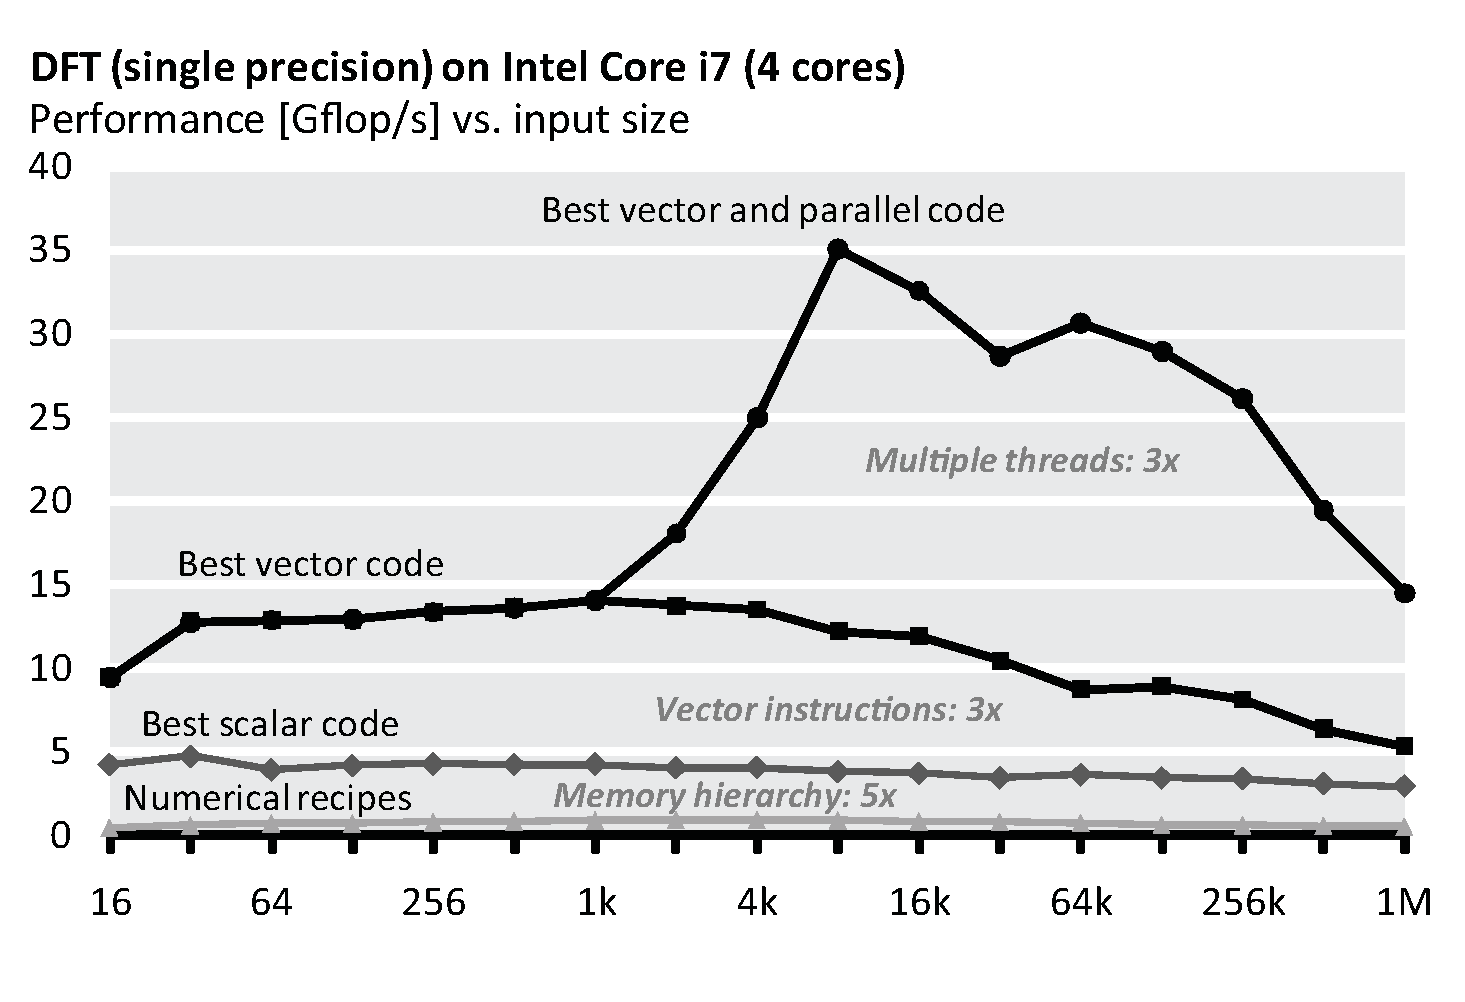
\includegraphics[scale=0.33]{dft-performance.eps}
  \caption{Performance of four single precision implementations of the
  discrete Fourier transform. The operations count is roughly the
  same. {\em The labels in this plot are too small.}\label{fftperf}}
\end{figure}



% References should be produced using the bibtex program from suitable
% BiBTeX files (here: bibl_conf). The IEEEbib.bst bibliography
% style file from IEEE produces unsorted bibliography list.
% -------------------------------------------------------------------------
\bibliographystyle{IEEEbib}
\bibliography{bibl_conf}

\end{document}

